\documentclass[sigconf]{acmart}

\AtBeginDocument{%
  \providecommand\BibTeX{{%
    \normalfont B\kern-0.5em{\scshape i\kern-0.25em b}\kern-0.8em\TeX}}}

\acmConference[VI1 '21]{VI1 '21:  Boids and Crowd Behaviour }{February 17, 2021}{Braga, PT}
\acmBooktitle{VI1 '21: Boids and Crowd Behaviour, February 17, 2021, BRAGA, PT}


\begin{document}

\title{Boids and Crowd Behaviour}

\author{Jos{\'{e}} Ferreira}
\affiliation{%
  \institution{Universidade do Minho}
  \city{Braga}
  \country{Portugal}}
\email{a83683@alunos.uminho.pt}

\begin{abstract}
With an increasing need to portray the real world in the realm of computer
graphics, the need to efficiently simulate complex natural behaviour became
more and more apparent. In this paper the state of the art of flocking,
swarming and crowd simulation will be explored.
\end{abstract}

\begin{CCSXML}
<ccs2012>
   <concept>
       <concept_id>10002944.10011122.10002949</concept_id>
       <concept_desc>General and reference~General literature</concept_desc>
       <concept_significance>300</concept_significance>
       </concept>
   <concept>
       <concept_id>10010147.10010371.10010352.10010378</concept_id>
       <concept_desc>Computing methodologies~Procedural animation</concept_desc>
       <concept_significance>500</concept_significance>
       </concept>
 </ccs2012>
\end{CCSXML}

\ccsdesc[300]{General and reference~General literature}
\ccsdesc[500]{Computing methodologies~Procedural animation}

\keywords{Boids, Crowd Behaviour, Crowd Simulation, Artificial Intelligence, State-of-the-art}

\begin{teaserfigure}
  \includegraphics[width=\textwidth]{images/Crowd_at_Knebworth_House_-_Rolling_Stones_1976.jpg}
  \caption{Crowd at Knebworth House - Rolling Stones 1976}
  \Description{Crowd watching a Rolling stones concert}
  \label{fig:teaser}
\end{teaserfigure}

\maketitle

\section{Introduction}
At first it was taught that nature was truly random and chaotic therefore
making it near impossible to accurately simulate and predict.
However, with the rise of scientific discovery and analysis, sets of
rules were discovered that describe the behaviours of nature.
This proves that nature, as complex as it appears at a first glance,
is actually a set of smaller rules interacting with each
other to create a bigger and more complex reality.

In the search to simulate complex structures and behaviours observed in reality,
the world of computer graphics also started to search for simple rules that closely
mimic reality. The main difference when compared with the scientific rules is that
there is a need for them to consume as little computational resources as possible.
Thus, for the most part, the main goal of the rules created for computer graphics
is to generate believable and visually pleasing results that appear reality-like
while consuming as little computational resources as possible.

One of the most relevant cases of this is the simulation of large groups of
animals or people. In this paper the evolution of the simulation of entities will
be explored, making brief references to the most relevant authors, leading into the
creation of entities capable of learning during a simulation. Then the most recent
algorithms for crowd simulation will be discussed and compared and their use cases
presented. Finally, what the future holds in this field will be discussed. 

\section{The Dawn of Boids}

The appearance of a large flock of birds might be mesmerising and appear truly
random at first as waves and direction changes propagate over the flock seemingly
without a origin or end. However, a flock is not a truly random system. Even tough
the position of each individual bird might not be predictable in the far future,
there is a high probability that, in the immediate future, any given bird will most
likely still be steering towards the same direction. Therefore, any attempt to simulate
how them behave cant be based on a random algorithm that arbitrary changes the
direction any given bird is flying.

After analyzing the behaviour of flocks and reaching this conclusions, Craig Reynolds
created the first instance of a boid in 1986\cite{Reynolds1987}. The term originates from
the contraction of the term ''bird-oid object'' meaning bird-like object and was used 
to describe a artificial life program that simulates the natural flight path of
a flock of birds. This type of program is generally called artificial life program
due to the fact that it seeks to recreate and simulate the interactions between animals
and the interaction of animals with the environment.

The creation of this program was considered a turning point in computer graphics
since up to that point the behaviour of a flock of birds was recreated by manually
defining the path of each bird one by one. This old method was extremely time
consuming and often produced sub-par results. The new method however, aimed to solve this
problems by instead defining the behaviour of each boid as a small set of rules that
defined steering behaviours in relation to the environment and the boids in the
immediate surrounding. This gave birth to procedurally generated animations that were
faster to implement and resulted in more realistic results.

Even tough the program has access to all the boid's position at any given time, the
information to process each rule is limited to only the nearby boids. This reduces 
the area of influence of each boid resulting in a more realistic result.
Additionally this method greatly reduces computation load since each boid only
looks at his vicinity and other boids inside of it.

Thus, based on the information they can collect each boid follows a set of three
different rules (Image \ref{fig:boid_rules}).

\begin{figure}[h]
  \centering
  \includegraphics[width=0.95\linewidth]{images/three_boid_rules.png}
  \caption{Three original rules for flock behaviour (\url{https://www.red3d.com/cwr/boids/}).}
  \Description{Visual representation of the three rules created by Craig Reynolds:
  Separation, Alignment and Cohesion}
  \label{fig:boid_rules}
\end{figure}

Firstly, each boid steers to avoid local flock-mates in order to avoid collisions
mid-air and ceate separation from nearby boids. Then the boid aligns itself with
the average heading of local flock-mates in order to follow the general direction
in which the flock is moving. Finally, so that the flock does not dissipate, the boid
steers towards the average position of local flock-mates.

This already creates realistic flocks with seemingly random waves that propagate over
time (Image \ref{fig:steamBoids}). However the flock does not interact with the environment
yet. In the original 1987 paper it is explored the possibility to add rules for object
avoidance and simple goal seeking. The later results in all the boids following a small
set of paths destroying the chaotic nature of a flock of birds.

\begin{figure}[h]
  \centering
  \includegraphics[width=\linewidth]{images/steam_boids.png}
  \caption{Boid simulation using Tabletop Simulator (\url{https://steamcommunity.com/sharedfiles/filedetails/?id=743303969})}
  \Description{Computer render with boids flying over the sunset}
  \label{fig:steamBoids}
\end{figure}

Ultimately this new development in computer graphics culminated in the creation of a
short film called ''Stanley and Stella in: Breaking the Ice''\cite{StanleyStella1987}.
In this short, a micro ecosystem exists inside a semi-transparent glass sphere half
filled with water. Under the water a school of fish swim around in a natural way avoiding
rectangular objects and above the water a flock of birds flies avoiding cylindrical
objects (Image \ref{fig:StanleyStellaBoids}). The short follows the story of Stanley
the bird and Stella the fish falling in love but being unable to meet face to face
due to a tick sheet of ice that formed on the water\cite{StanleyStellaIMDb}.
The first version of the film did not gain much traction outside of the computer
graphics field. Nevertheless, after a tonal shift provided by a new, less somber, Jazz
soundtrack and a renaming to ''Love Found'' this film actually gained a certain cult
following amongst certain film enthusiasts that enjoy the aesthetic of computer
generated graphics of this era and was even aired several times on television. Now
it is available on several video sharing platforms like youtube.

\begin{figure}[h]
  \centering
  \includegraphics[width=\linewidth]{images/stanley-and-stella-in-breaking-the-ice.jpg}
  \caption{Stanley and Stella in: Breaking the ice\cite{StanleyStella1987} scene}
  \Description{Computer render of a flock of orange and yellow birds flying inside a
  glass dome avoiding blue cylindrical objects }
  \label{fig:StanleyStellaBoids}
\end{figure}

Even tough the graphics do not hold up today this short film came as a turning point
in computer graphics and computer animation and represents one of the first instances
of realistic procedurelly generated animation since both the fish and the birds use
the revolutionary technology developed by Craig Reynolds to streamline the creation
of this complex animations for the time.

\section{Creation of Boid Individuality}

After the breakthrough created by Craig Reynolds the study of boids gained great
traction amongst the computer graphics field. This is due to the fact that
one of the goals of computer engineering that is transversal to all of it's fields is
the search of simplicity and efficiency. Thus, it is far better for a task to be
performed automatically by a computer than to be painstakingly created by a artist,
programmer or designer. This goal perfectly fits the concept of the simulation of schools
of fish or flocks of birds with the use of Boids.

Even tough initially the work of Craig Reynolds was targeted towards simply representing
in a way that seems credible the real world without necessarily having scientific
accuracy, the scientific community quickly realised that the possibility of running
simulations over the behaviour of animals could lead to scientific breakthroughs.
For example, it could become possible to study the reaction of animals to the
introduction of an invasive species.

After realizing that there were several applications for the ability to simulate the
behaviour of large groups of animals outside of simply graphically representing them in
a believable way, a need to simulate the behaviours of more complex entities started
to appear. However the boids created by Craig Reynolds are simply to restrictive to recreate
the real world realistically.

In order to overcome the hurdle posed by the simplicity of the boid algorithm a
incessant search for different paradigms for the simulation of large number of
entities started.

The work of Craig Reynolds regarding the simulation of school of fish was greatly
built upon in 1994 by Xiaoyuan Tu, Demetri Terzopoulos and Radek Grzeszczuk
\cite{Terzopoulos94artificialfishes:}. This team
was most notably able to greatly increase the complexity of each boid and how it
interacts with the environment. Each boid was previously simply a three dimensional
model with a default swim animation attached to a point that followed a predetermined
set of rules.
This basic system was changed into a structure of muscle and actuators controlled by
a larger set of behaviour routines that can be optimized overtime by an artificial
intelligence algorithm. To further add to the individuality of each boid a set of
habits of each individual are taken into account when interacting with the
environment. To further improve the realism, the number of sensors and data
available to the boid was increased. Finally, physical properties were added to
the environment so that, for example, the movement of a fish under water
interacts following the hydrodynamic principles (Image \ref{fig:fishControlFlow}).

\begin{figure}[h]
  \centering
  \includegraphics[width=\linewidth]{images/fish_learning.png}
  \caption{Control and information flow in artificial fish(from the original article\cite{Terzopoulos94artificialfishes:})}
  \Description{Representation of the control flow described above}
  \label{fig:fishControlFlow}
\end{figure}

Furthermore, the demonstration used
to visually represent the new theory also showed the great development in computing
power and graphical fidelity (Image \ref{fig:smartFish}).

\begin{figure}[h]
  \centering
  \includegraphics[width=\linewidth]{images/smart_fish.png}
  \caption{Artificial fishes in their physics-based world (taken from the original paper\cite{Terzopoulos94artificialfishes:})}
  \Description{A small group of fishes swims underwater close to the sea bed. There are
  three different species visible: a striped yellow and grey, a blue, and a striped orange and grey}
  \label{fig:smartFish}
\end{figure}

\section{Categorization of Algorithms}

Even tough this algorithm represented a massive breakthrough in the realistic representation
of large groups of varied entities, the underlying logic is still similar: Each entity's
interaction with the environment and other entities is individually computed. 

With the development of new algorithms that, for example, focused more on the global
flow of the crowd, the need to classify them surfaced. Thus, a set of three categories
where created to define the possible approaches to the problem of Crowd simulation
%(Table \ref{tab:categoriesCrowd})
: Agent-based Approach, Flow-based Approach and Entity-based Approach \cite{Zhou2010}.

All the algorithms that fall under the category of Agent-based approach are described as
a set of autonomous interacting individuals with a certain level of intelligence that react
to the environment and each other based on a set of rules. This rules can change during
the simulation based on the interaction of the entities with the environment giving them
the ability to learn during the simulation. This gives complete control to the researcher
making this type of simulation possibly the most realistic in modeling the behaviour albeit
the most computationally expensive. The boid algorithm after being improved in 1994 is an
example of a Agent-based approach.

By contrast, Flow-based Approach focuses on simulating a crowd as a whole. Thus, when this type
of simulation is used, the focus is usually on how the crowd reacts and interacts
with the environment and flows through it in the general sense. For example, this simulation is
often used to simulate how a large crowd flows through a small opening like a door
(Image \ref{fig:crowdFlow}). Interestingly this algorithm often
borrows elements from the study of fluid dynamics\cite{YUAN20114210}. Since this method mimics
the flow of a crowd the individuality of each entity is mostly nonexistent leading to
the lowest cost per entity of all of the three approaches. This model is mainly used to
simulate large sets of elements in a small time frame.

\begin{figure}[h]
  \centering
  \includegraphics[width=0.95\linewidth]{images/crowd_flow.png}
  \caption{Crowd Flow during Black Friday in 2011 (\url{https://www.youtube.com/watch?v=DigiWS1YhxI})}
  \Description{A large crowd is trying to enter a store through a small door}
  \label{fig:crowdFlow}
\end{figure}

Finally, the entity-based approach can be considered a middle ground between the previous
approaches. A set of immutable global laws are created that rule the way the entities behave.
This rules cannot be changed during the simulation making the entities unable to learn
and improve during the simulation. This type of algorithm is ideal to simulate small to
medium crowds in short time frames. Also, the increased simplicity when compared with the
Agent-based approach greatly reduces the computational cost per entity making it
a middle ground in terms of computing power between the previous methods.

%\begin{table}[h]
%  \caption{types of approach}
%  \label{tab:categoriesCrowd}
%  \begin{tabular}{cccl}
%    \toprule
%    Categories & Time Frame & Crowd Size & Load per entity\\
%    \midrule
%    Agent-based & any & any & highest\\
%    Flow-based & short & large &lowest\\
%    Entity-based & short & small &  \\
%  \bottomrule
%\end{tabular}
%\end{table}

\section{Real World Applications}

Surprisingly, even tough there have been many breakthroughs in the research of  crowd
simulation, in many areas, the original algorithm crated by Craig Reynolds is still used
to this day mostly unchanged. This approach still shines in cases where there is a need
for simple and fast computations to create a scene. The two most prominent use cases of
this technology to this day are video games and background CGI in movies. In
recent years there has been a shift towards more complex algorithms in the movie
industry mainly in blockbuster movies.

Apart from leisure activities, there are some real world applications that have direct impact
in the quality of life of the human population. For example, there are many areas in the design
of modern cities that require the simulation of large crowds to ensure that it is up to the
required standards. Urban planning, Evacuation Handling and Law Enforcement are great examples of this.

\subsection{Video Games}

One of the most well know examples of Boids in a video game is present in Half-Life
released in 1998. In this game, flocks of green and orange flying monsters (Image
\ref{fig:halfLifeBoid}) can be seen near the end of the game when the player enters
a region known as Xen. This flocking behaviour uses a simple algorithm very similar to the
one developed in 1987 by Craig Reynolds\cite{Half-LifeWiki}. After
analysing the code of the game it was discovered that there were plans to add a second
yellow variant of this entity capable of more advanced interactions with each other, including
the creation of a small ecosystem with predators and prey. However this was considered
unnecessarily advanced and too computationally expensive in a performance critical program
such as a video game and eventually the concept was scrapped.

\begin{figure}[h]
  \centering
  \includegraphics[width=0.95\linewidth]{images/half-life_boids.jpg}
  \caption{Flocking Behaviour in Half-Life}
  \Description{Green creatures with a shape similar to a tailless sting ray flock above green fields}
  \label{fig:halfLifeBoid}
\end{figure}

The limits of the hardware at the time was also one of the factors that made many developer
choose to use procedurelly generated flight paths instead of having a large set of pre-generated
flight paths for the birds: it is actually more space efficient to save the code that creates
animations rather than the flight paths themselves

\subsection{Film, Cinema and Movies}

Boids are often used in the case of swarm or flock simulation in movies\cite{BAJEC2009777}. A great example of this
is the 1992 film ''Batman Returns'' directed by Tim Burton. In this movie swarms of bats that use the boid
algorithm were used in several scenes (Image \ref{fig:batmanSwarm}). Since at this time there had been a
great jump in computation power and investment from the movie studios into computer generated graphics,
the bats in this movie appear much more life like when compared with the movie created with the help of
Craig Reynolds.

\begin{figure}[h]
  \centering
  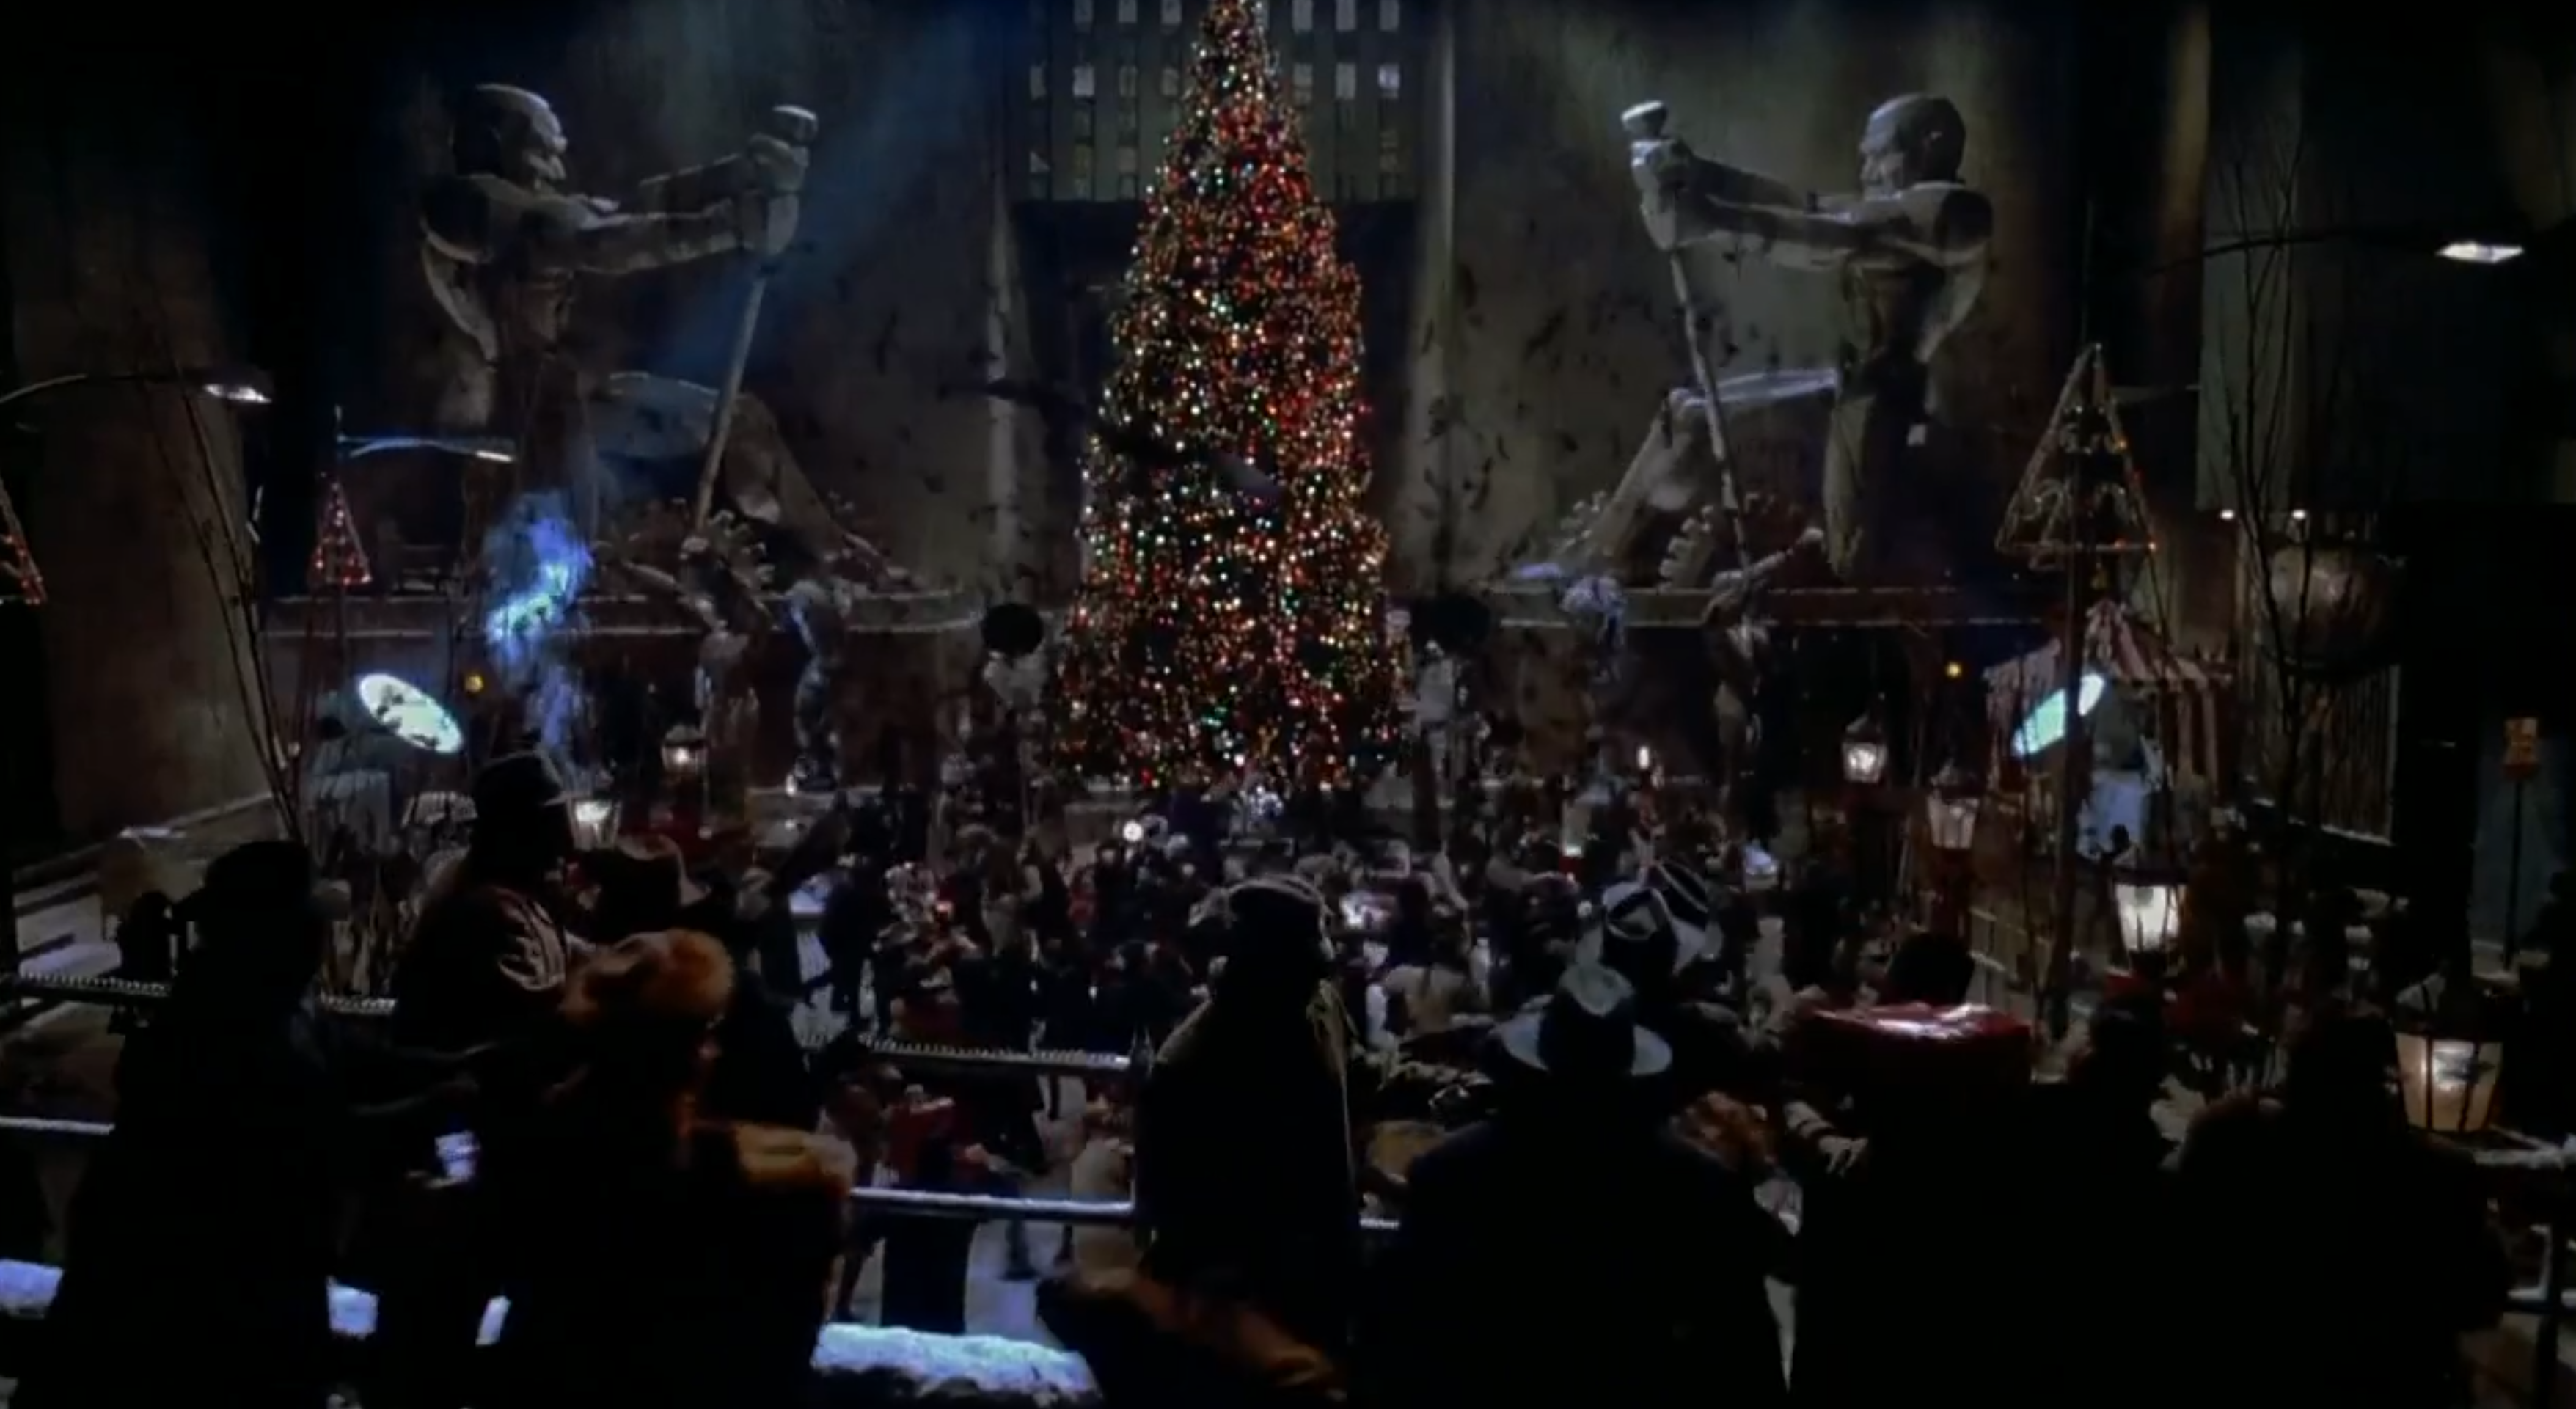
\includegraphics[width=\linewidth]{images/batman_bats.png}
  \caption{A swarm of bats using boid algorithms in 1992 ''Batman Return's''}
  \Description{swarm of bats terrorizes citizens inside a city hall in the 1992 film Batman Return's}
  \label{fig:batmanSwarm}
\end{figure}

However, sometimes such simple algorithms are not enough to simulate the more complex scenes.
Usually in the simulation of armies clashing in a fierce battle, it is not enough to have them
simply avoid each other and their surroundings. Each entity has to have a goal and a varied set
of actions they can take to create the maximum variety possible in a scene containing thousand of
entities\cite{Davis2003MultipleAS}. One of the most well know example of such grandiose battles
containing upwards of fifty thousand soldiers were ''The Lord Of the Rings'' trilogy
(Image \ref{fig:lotr}. The production of this movies used an already existing program to develop
the animations. Yet, what made it stand from the rest was the much larger number of individual
animations each entity could perform based with it's interaction with the environment.

\begin{figure}[h]
  \centering
  \includegraphics[width=\linewidth]{images/lotr.jpg}
  \caption{Battle of Helm's Deep in ''Lord of the Ring: The Two Towers''}
  \Description{A giant orc army is storming a walled of city}
  \label{fig:lotr}
\end{figure}

\subsection{Drone Swarms}

Recently there have been many examples of shows and popular sports events
were the fireworks are changed to a more  Eco friendly solution based on swarms of drones with a multi-color light source
attached to the base. This allows to create extreme complex animations in the night sky that would be otherwise utterly
impossible to recreate with traditional means (Image \ref{fig:drones}).

\begin{figure}[h]
  \centering
  \includegraphics[width=\linewidth]{images/drone_fireworks.png}
  \caption{Swarm of drones creating a running animation}
  \Description{Swarm of drones creating a running animation}
  \label{fig:drones}
\end{figure}

To create each figure a drone has a target destination where he has to go to without entering in a collision route
with any of the thousands of other drones that are also trying to reach their respective destinies. To achieve this
swarm simulation algorithms similar to the one developed for boids are used.

This area of robotics is called Swarm Robotics and there are many uses outside of simple entertainment for this
revolutionary technology. For example, there are currently many teams dedicated to the study of swarms
of flying or ground drones capable of finding victims in a catastrophe\cite{2014outdoor}, returning to base when there
is a need for repairs or recharging (Image \ref{fig:recharging}) and entering hostile environments.

\begin{figure}[h]
  \centering
  \includegraphics[width=\linewidth]{images/RechargingSwarm.jpg}
  \caption{Swarm of open-source Jasmine micro-robots recharging themselves [CC BY-SA 3.0]}
  \Description{Swarm of open-source Jasmine micro-robots recharging themselves}
  \label{fig:recharging}
\end{figure}

\subsection{Urban Planing}

Urban planing of a large city covers a wide area of topics. There is a need to define how the land
is to be divided and used in the long term and decide how all the infrastructures in the city will
be built accounting for future changes in population density and technologies.

Infrastructure planing can be divided in two broad topics: Areas that directly influence how people
navigate through a city and areas that do not. Examples of areas that do not influence how people
navigate a city include water, gas and electrical grid. Examples of areas that do influence how people
navigate a city are transportation and roads\cite{urbanPlanning}.

Since crowd simulation is better suited to areas that directly influence how people move people,
the later is the area that mostly benefits from crowd simulation.

When compared with mathematically calculating the maximum possible flow in a given intersection or roundabout,
the ability to simulate different flows, road designs and time frames with the press of a button paints a much
more realistic representation of the impact of a given alteration on the real world. Thus, when applied in a
large scale, urban planing allied with crowd simulation can represent a great improvement on the quality of life. 

One of the greatest example of a city wide optimization of infrastructures comes from from the ''prototype
city of the future'' that is being created by Toyota in Japan\cite{wovenCity}. Toyota is calling the city
''Woven city'', a reference to how different types of roads dedicated to different type of traffic where
optimized as much as possible to create a woven network of roads, parks and buildings that maximise safety,
flow and well-being of the citizens (Image \ref{fig:woven}). The company expects that the city will house
over two thousand people by the end of 2021.

\begin{figure}[h]
  \centering
  \includegraphics[width=\linewidth]{images/woven_city.jpg}
  \caption{Woven City Concept presented bu Toyota at CES 2020}
  \Description{Computer generated City square with Green pathways}
  \label{fig:woven}
\end{figure}

Toyota's claims are not unfounded, most experts believe that the city of the future is in fact an interconnected
mesh of sustainable services and resources powered by constant developments in the capability to simulate human
behaviour and cater to it.

\subsection{Evacuation Handling}

If Urban Planing is Crowd simulation applied in the macro scale, then Evacuation Handling is the micro scale.
Instead of simulating how an entire city behaves during the day or rush-hour, evacuation handling powered by
crowd simulation focuses how a subset of a city, usually a building or road section, reacts during a catastrophe
in a small time frame\cite{Evacuation}.

This simulations have to be often altered to accurately represent how a human behaves during stressful
events\cite{evacuationRobots}.
Firstly, when scared, people tend to behave as a herd following the person immediately in front of them.
Secondly, not everyone knows the space they are navigating in the case of an emergency. Thus, they do
not know what kind of hazards and obstacles can be on the way.
This leads to situations in which a crowd is trying to rush to the same exit while another exit a couple of
meters away is completely deserted (Image \ref{fig:crowdBuilUp}).

\begin{figure}[h]
  \centering
  \includegraphics[width=\linewidth]{images/crowd_escape.png}
  \caption{Crowd Simulation trying to escape a smoke filled room}
  \Description{A crowd is trying to escape a smoke filled room but the herding behaviour of people in panic
  prevents them from equally dividing themselves between the two available exits}
  \label{fig:crowdBuilUp}
\end{figure}

If this stampeding behaviour  of humans in panic  can be precisely replicated in a simulation, parameters
can be changed in order to create better evacuation plans for a building and save lives in a catastrophe.
Thus, there has been a lot of research effort put into this area resulting in many programs capable of
simulating and optimizing evacuation routes in a building (Image \ref{fig:crowdFire}).

\begin{figure}[h]
  \centering
  \includegraphics[width=\linewidth]{images/evacuation_simulation.jpg}
  \caption{Simulation of an Emergency Evacuation due to a fire }
  \Description{A crowd is trying to escape a building in flames}
  \label{fig:crowdFire}
\end{figure}

\subsection{Law enforcement}

Law enforcement often has to deal with crowds in panic and herd behaviour similar in many ways with the one
present in Evacuation Handling. Examples of such parallels are protests and catastrophe relief were
in both a herd mentality can be observed in the movement of people. In a protest people tend to follow the
person they perceive as a leader, such as the one holding the placards or the megaphone. On the other hand,
in catastrophe relief people tend to be disoriented and follow the person immediately in front of them.

To better train police officers, firefighters and military to deal with mobs and crowds, simulations can be
used to train how each group can help calm and direct people to act as effectively as possible.

\begin{figure}[h]
  \centering
  \includegraphics[width=\linewidth]{images/chile_firefighters.jpg}
  \caption{Firefighters after a 6.2-magnitude earthquake in Chile (\url{https://i.dailymail.co.uk/i/pix/2016/08/24/22/378E249600000578-3755722-image-a-3_1472075559182.jpg})}
  \Description{Simulation of a group of policemen standing in front of a protesting crowd}
  \label{fig:firefighters}
\end{figure}

In fact, there are already examples of this in the real world\cite{SIDIROPOULOS2020100009}. For example, Rotterdam's Police
and the Dutch Government have developed a real time simulation of riots and protests in conjugation with VSTEP
called ''VSTEP Crowd Control Trainer''\cite{crowdControl}(Image \ref{fig:police}) that accurately represents how
a agglomerate of people reacts to police intervention.

\begin{figure}[h]
  \centering
  \includegraphics[width=\linewidth]{images/crowd_control.png}
  \caption{Crowd Control Trainer example\ref{fig:police}}
  \Description{Simulation of a group of policemen standing in front of a protesting crowd}
  \label{fig:police}
\end{figure}

Nowadays this tool is used to train more efficient police brigades in three different fields. The ability to
manage a crowd by creating order, the ability to control a crowd and maintain order and the ability to deescalate
rising tensions in order to prevent riots and violence, allowing very varied simulations including the simulation
of opposing groups that have to be guided in order to avoid each other (e.g. football supporters).


\section{Conclusion and the Next Step}
The study of boids and crowd behaviour and subsequent simulation of them is a field of real time computer graphics with
many real life applications. From leisure activities,like movies and video games, to critical activities that can
save lives or help save the planet by reducing pollution, like evacuation handling or urban planning. Thus, making
this an area that directly impacts human's quality of life. 

This rise in interest from many areas will surely will surely not stop in the foreseeable future creating a snowball
effect that will result in a complete revolution of how it is implemented and created in a near future.

One of the hot topics is the ability to have each entity behave based on a complex neural network effectively
increasing the autonomy and learning abilities. Currently this technology is far from being wide spread and
capable of being computed in real time. However, with a heavy investment from GPU manufacturers into graphics
cards with an increased neural network computing capacity\cite{nvidiaAI,amdAI} it is not difficult to imagine
that crowd simulations in the near future will be powered solely by complex neural networks.

This performance boost comes mainly from the implementation of tensor cores. These are dedicated areas of memory
for matrix operations that support the most common operations, such as matrix multiplication, that are common in both
computer graphics and AI leading to an increase in throughput up to 32 times (Image \ref{fig:tensorcore}).

\begin{figure}[h]
  \centering
  \includegraphics[width=\linewidth]{images/tensorcores.jpg}
  \caption{Nvidia Tensor core performance comparison for dotprod}
  \Description{Comparison of dotprod performance in diferent Nvidia architectures}
  \label{fig:tensorcore}
\end{figure}

Although neural networks can lead to a more realistic simulation to be used in critical areas,  this bleeding-edge
technology will surely make its way into leisure activities to also improve the quality of movies and video games
and create more immersive experiences were the world fells truly alive when observed.

\bibliographystyle{ACM-Reference-Format}
\bibliography{sample-base}

\end{document}
\endinput